\subsubsection{Linux}

\paragraph{Question 1} (Linux). Un enseignant partage des fichiers avec ses étudiants en les plaçant dans un répertoire Linux de son département accessible publiquement. Un jour, il réalise qu'un fichier placé la veille est en écriture pour tous. Il modifie les permissions et vérifie que le fichier est identique à la version d'origine. Le lendemain, il découvre que le fichier a été modifié. Comment est-ce possible et comment aurait-on pu l'empêcher ?
\color{reponse}
\begin{itemize}
	\item Un étudiant a pu garder le fichier ouvert avant et pendant que le prof modifiait les permissions, puis il a sauvegardé le fichier. Le professeur aurait dû supprimer le fichier puis placer une copie du fichier maître dans le répertoire publique.
\end{itemize}
\color{black}



\paragraph{Question 2} (Linux). Est-il possible qu'avec l'algorithme buddy pour l'allocation de mémoire physique en Linux que deux blocs de mémoire adjacents, libres et de même taille, coéxistant sans être réunis en un bloc de taille double ? Si oui, expliquer comment. Sinon, prouvez-le.
\color{reponse}
\begin{itemize}
	\item C'est possible si les deux blocs ne sont pas des buddies. Prenons l'exemple de la figure \ref{Deroulement du buddy algorithm} (e).
\begin{figure}[p]
	\centering
	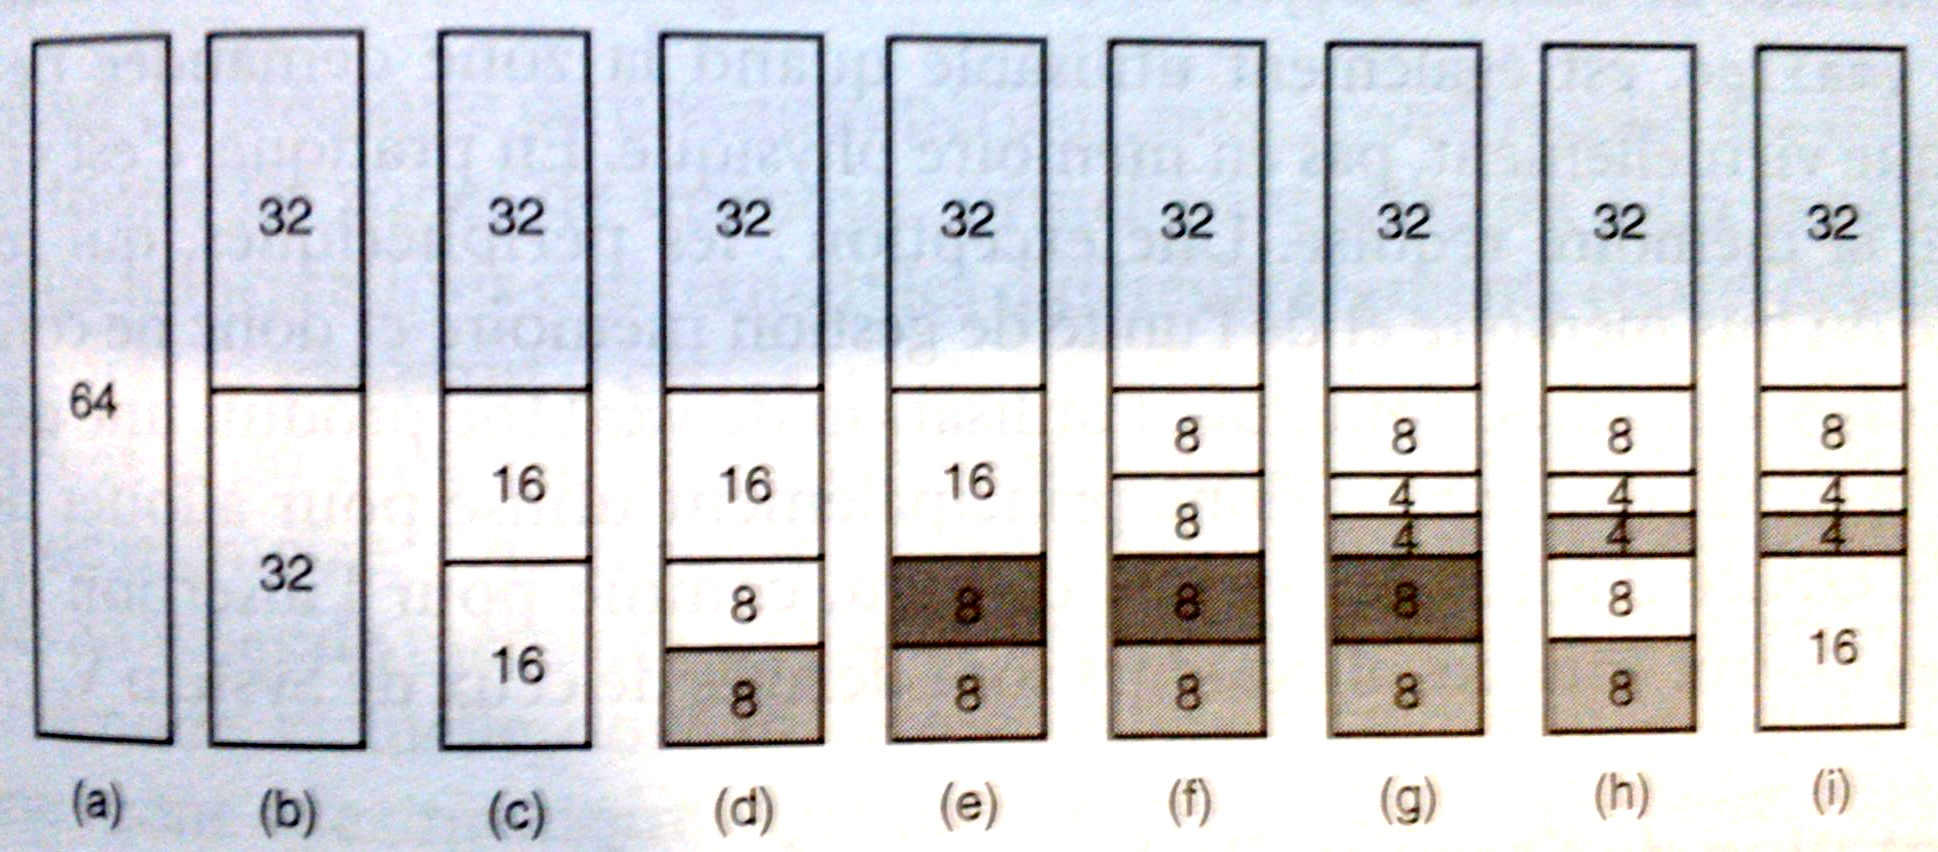
\includegraphics[scale=0.2]{images/buddyalgo.png}
	\caption{\label{Deroulement du buddy algorithm} Déroulement du \textit{buddy algorithm}.}
\end{figure}
Deux nouvelles requêtes entrent pour 8 pages chacune. À ce point, les 32 pages du bas sont la propriété de quatre utilisateurs différents, possédant 8 pages chacun. Les utilisateurs 1 et 2 libèrent leurs pages, mais les utilisateurs 0 et 3 conservent les leurs. Cela produit une situation dans laquelle 8 pages sont utilisées, 8 pages sont libres, 8 pages sont libres et 8 pages sont utilisés. Ces deux blocs adjacents de taille égale ne peuvent pas fusionner parce qu'il ne sont pas des buddies.
\end{itemize}
\color{black}



\paragraph{Question 3} (Linux). Quand un nouveau processus est crée un nombre entier lui est attribué pour PID. Est-ce suffisant d'avoir un compteur dans le noyau qui s'incrémente à chaque création de processus et qu'on utilise pour distribuer les PID ? Justifiez votre réponse.
\color{reponse}
\begin{itemize}
	\item Non ce n'est pas suffisant, tout PID doit être unique. Tôt ou tard, le compteur boucle et revient à 0. Il monte ensuite à 15, par exemple. S'il se trouve que le processus 15 a été démarré il y a plusieurs mois mais qu'il s'exécute toujours, on ne peut pas assigner 15 à un nouveau processus. Ainsi, une fois que le PID a été choisi par le biais du compteur, on doit parcourir la table des processus pour vérifier si le PID est toujours exploité.
\end{itemize}
\color{black}



\paragraph{Question 4} (Linux). Quel est le fonctionnement de l'ordonnanceur de processus et des threads sous Linux, quel est le principe des 280 têtes de listes \textit{active / expired} ? Comment évoluent les priorités?
\color{reponse}
\begin{itemize}
	\item   
\end{itemize}
\color{black}



\paragraph{Question 5} (Linux). Libérer la mémoire d'un processus quand ce dernier passe dans l'état zombie a-t-il un sens ? Justifiez votre réponse.
\color{reponse}
\begin{itemize}
	\item Oui. Il ne peut plus s'exécuter, donc plus sa mémoire retourne rapidement sur la liste libre, mieux c'est.
\end{itemize}
\color{black}



\paragraph{Question 6} (Linux). En général, pensez-vous que les \textit{daemons} ont une priorité supérieure ou inférieure à celle des processus interactifs ? Pourquoi ?
\color{reponse}
\begin{itemize}
	\item En général, les \textit{daemons} s'exécutent à l'arrière-plan pour effectuer des tâches telles que l'impression et l'envoi de courrier électronique. On leur attribue une priorité faible et ils profitent du surplus de temps UC que les processus interactifs n'emploient pas.
\end{itemize}
\color{black}



\paragraph{Question 7} (Linux). Dans chaque entrée de la structure de tâche, on trouve le PID du processus parent. Pourquoi ?
\color{reponse}
\begin{itemize}
	\item Quand le processus quitte, le parent reçoit l'état de sortie de son enfant. On a besoin du PID pour identifier le parent afin que l'état puisse être transféré au processus correct.
\end{itemize}
\color{black}



\paragraph{Question 8} (Linux). Quand on lit un i-node sur disque lors de l'ouverture d'un fichier, il est plaçé en mémoire dans la table des i-nodes. Cette table possède certains champs qui ne figurent pas sur disque. L'un d'eux est un compteur mémorisant le nombre de fois que l'i-node a été ouvert. Pourquoi ce champ est-il nécessaire ?
\color{reponse}
\begin{itemize}
	\item Lorsque l'on ferme un fichier, le compteur de son i-node en mémoire est décrémenté. S'il est supérieur à zéro, on ne peut pas supprimer l'i-node de la table, puisque le fichier est toujours ouvert dans un processus. C'est uniquement quand le compteur atteint zéro que l'ont peut supprimer l'i-node. Sans le compte des références, le système ne pourrait pas savoir quans supprimer l'i-node de la table. Créer une copie séparée de l'i-node chaque fois que l'on ouvre le fichier ne fonctionne pas, dans la mesure où les modifications apportées à une copie ne seraient pas visibles sur les autres.
\end{itemize}
\color{black}



\paragraph{Question 9} (Linux). Est-il possible de faire un \textit{unlink} d'un fichier qui n'a jamais été lié ? Que se passe-t-il ?
\color{reponse}
\begin{itemize}
	\item Le fichier est simplement supprimé. C'est la méthode classique (la seule) pour supprimer un fichier.
\end{itemize}
\color{black}



\paragraph{Question 10} (Linux). Donnez le fonctionnement du système de fichier ext2 du noyau linux, exprimez la taille maximale d'un fichier en fonction de la taille des blocs (b un nombre d'octets) et pour des adresses de 32 bits.
\color{reponse}
\begin{itemize}
	\item 
\end{itemize}
\color{black}